\documentclass[10pt,twocolumn,letterpaper]{article}
\usepackage[margin=2.5cm]{geometry}
\usepackage{times,epsfig,graphicx,amsmath,amssymb}
\usepackage{algorithm, algorithmicx, algpseudocode, subcaption, float}
\usepackage[breaklinks=true,colorlinks=true,bookmarks=false]{hyperref}
\date{}

%%%%%%%%%%%%%%%%

\title{Synthetic Bokeh from Paired Semi-Stereo Portrait Images}

\author{%
John Gibson\\
{\tt johngibson@wustl.edu}
}


\begin{document}
\maketitle

\begin{center}\textbf{Abstract}\\~\\\parbox{0.475\textwidth}{\em
    % Abstract goes here
    Portrait images generally make use of background blur to isolate a subject and create visual interest.
Professional photographic systems make use of large sensor sizes, long focal lengths of 50mm or more, and wide lens apertures of f/2.8 or wider
to achieve this effect. However, the small size and wide angle lens of personal cell phone cameras cannot reliably create this effect,
and thus much work has been done to recreate this effect using postprocessing. This project uses paired images in relatively stereo configuration
(e.g. not completely vertically aligned) to compute a depth map, detects faces in the input images to determine the face disparity value, and
then blurs the input image based on the computed disparities. In addition, different methods of computing the disparity map and blurring the
output image are tested and compared.

}\end{center}

\section{Introduction}

\par Bokeh (BOW-keh), or background defocus, has long been a staple of photographic portraits. Certain lenses and camera systems are prized for their ability
to render out-of-focus elements of a frame in an aesthetically pleasing way, and the most prized lenses can sell for thousands of dollars. Professional
camera systems achieve pleasing and strong background defocus using large sensor sizes and lenses with wide apertures and long focal lengths.

\begin{figure*}[!t]
    \begin{center}
        \includegraphics[width=3.0in]{resources/bokeh_example.jpg} % Place holder, replace with \includegraphics, etc.
    \end{center}
    \caption{\small A portrait with strong bokeh, taken at a focal length of 56mm, an aperture of 1.2, and a sensor size of 23.5 mm x 15.6 mm. Note the large light balls in the background, which is a characteristic of true bokeh.}
    \label{fig:bokehexample}
\end{figure*}

\par However, cell phone cameras with small sensor sizes (e.g. 1/2.3" or 1/1.7") and short focal lengths cannot accurately reproduce such an effect with the desired
intensity for portraits. Therefore, much work has been done to recreate bokeh using computational post-processing effects. Most modern cell phones, including the
Apple iPhone, Google Pixel, and Samsung Galaxy series come equipped with a "portrait mode" that reporoduces this background blur in software. However, these
devices often make use of specialized hardware or rolling camera buffers to achieve this effect. This project aims to create a tool to create convincing bokeh from semi-stereo
images that are not perfectly aligned.

\section{Background \& Related Work}
\par Multiple phone camera software producers have attempted this effect, most notably the Google Pixel. The Pixel's sensor is comprised of dual-pixel elements,
which consist of two independent photodiodes per photosite that receive light at different angles.
Taking a picture effectively creates two different images, a left image and a right image, which can be used in any stereo disparity matching algorithm to
create a depth map. The subject is then segmented from the scene using a neural network based on U-Net, and the disparity for that region is set to 0. Then,
the other pixels of the depth map are scaled according to the difference between the pixel value and the original depth of each pixel in the subject region.
Call the resulting depth map $D'$.
Then, each pixel is blurred in a hierarchical manner, according to the pixel's value in $D'$, with pixels with larger values in $D'$ being blurred with more
intensity. This approach is detailed in \cite{wadhwa_et_al_2018}. A special depth map estimation technique was developed by Google \cite{barron_adams_shih_hernandez_2015}
which takes advantage of advances in fast bilateral filtering to enforce bilateral properties on the depth map, produceing smooth, edge-aware disparity regions.
The iPhone uses a similar approach, except it does not have a dual-pixel sensor like the Google Pixel, and instead uses both the 2x telephoto lens and wide-angle lens
as input to a trained convolutional neural network for depth estimation. The implementation details of Apple's portrait mode are hidden from the public, however, so not
much is known about the network structure or other algorithms used.

\par Both of these methods require perfectly aligned stereo images, whether from multiple physical cameras or using the dual-pixel sensor.
In this work, we aim to relax this constraint and allow images which are only semi-stereo; that is, not perfectly aligned horizontally or vertically,
to be used to compute the depth map. In addition, much progress has recently been made in monocular depth estimation using deep convolutional neural
networks, which use information in the scene to estimate depth. This would allow realistic background blur from only a single image!
Numerous pre-trained models are available, and for this work we use a network called monodepth2 from Niantic, Inc. and Gabriel Brostow \cite{monodepth2}.

\section{Proposed Approach}

\begin{figure}[t]
    \begin{center}
        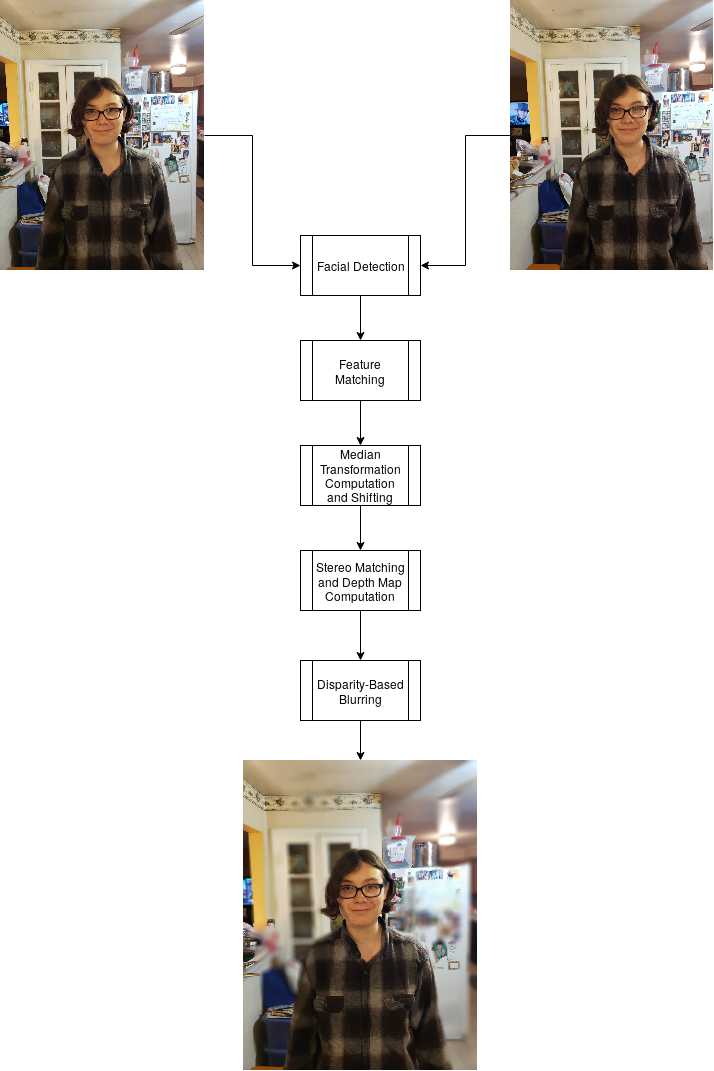
\includegraphics[width=2.95in]{resources/portrait_mode.png} % Place holder, replace with \includegraphics, etc.
    \end{center}
    \caption{Proposed pipeline for semi-stereo portrait mode. Two unaligned input images are run through a face detection algorithm to find the location of the face and are aligned using feature matching.
    A depth map is then generated from the aligned images using a stereo disparity matching algorithm such as SGBM or Fast Bilateral Stereo Matching. Finally, the output is blurred, with regions farther away
    from the calculated disparity of the face blurred with a higher intensity.}
    \label{fig:pipeline}
\end{figure}

The general proposed approach is depicted in Figure \ref{fig:pipeline}.

\subsection{Face Detection}

Facial detection was implemented using OpenCV's pre-trained Haar cascade model, based off of the method of Viola and Jones \cite{viola_jones_2004}.
Face detection was performed on both images as a sanity check, and the position of the face in the first input image is saved.

\subsection{Feature Matching and Median Feature Transformation}

AKAZE \cite{alcantarilla_nuevo_bartoli_2013} feature detection was performed using the OpenCV implementation, and features were matched using
OpenCV's brute force matcher (BFMatcher). Then, the following procedure was performed:
\begin{enumerate}
    \item Obtain the top two matches in the right image for the feature in the left image and perform a distance ratio test to ensure the uniqueness of the match. If it does not pass, remove it from the matches.
    \item Compute the angle between each pair of matched features with respect to the x-axis of the image and sort them in non-decreasing order with respect to this value.
    \item Using a user-configurable parameter $m$, take the middle $m\%$ of matches and compute their average for $\Delta x$ and $\Delta y$, rounded to the nearest whole number.
    \item Shift the right image by $\Delta y$ along the y-axis such that the features are aligned (roughly) horizontally.
\end{enumerate}

This procedure aligns the images for stereo matching along the horizontal axis.

\subsection{Stereo Matching and Depth Map Computation}
Three different methods of stereo matching were tested:
\begin{enumerate}
    \item Semi-Global Matching using Mutual Information, based off of Hirschmuller 2007 \cite{hirschmuller_2007}, using OpenCV's implementation.
    \item Fast Bilateral-Space Stereo \cite{barron_adams_shih_hernandez_2015}, based off an implementation by Toon Van den Zegel \cite{fast_bilateral_stereo} and modified for stability and performance.
          This method transforms the image into "bilateral space," in which pixel values are assigned to a small set of grid points in a lattice and blurred, then interpolated back into pixel space.
          Small blurs in bilateral space are equivalent to large, edge-aware blurs in pixel space, as the reinterpolation of the sparse points leads to close, similar regions of points containing the
          same blurring value. Optimization is performed in the bilateral space, with a loss function minimizing differences in pixel disparities based on their spacial and coloric affinities with some
          smoothness constraint. A domain transform filter is applied on the output for smoothing.
    \item Monodepth2 \cite{monodepth2}, an open-source monocular depth estimation network (only run on image 1). A simple server was implemented in Python using pynng and communicated with using nngpp in C++.
\end{enumerate}

Once the depth map for image 1 is computed, the depth of the face is calculated by averaging the depth values of 9 points in a 3x3 grid separated by $n$ pixels (default 100) that is centered in the middle of the detected face bounding box and rounded to the nearest integer.

\subsection{Hierarchical Disparity-Based Blurring}

\par A modified blurring algorithm of Barron et al. \cite{barron_adams_shih_hernandez_2015} was implemented and used for disparity-based blurring, which is outlined in Algorithm \ref{alg:blur}.

\begin{algorithm}[h]
    \caption{Hierarchical Disparity-Based Blurring}
    \label{alg:blur}
\begin{algorithmic}
    \State $I_n \gets 0$
    \State $I_d \gets 0$
    \State $\text{Normalize } D \text{ from 0 - 255}$
    \State $\hat{D} \gets \text{abs}(D - d_{\textit{face}})$
    \For{$d = \min \hat{D} : \max \hat{D}$}
        \State $A \gets  \hat{D} = d$
        \State $B \gets I \times A$
        \State $r \gets m \max{(d - z, 0)} \text{ rounded to nearest odd integer}$
        \State $A_b \gets \text{blur}(A, r)$
        \State $B_b \gets \text{blur}(B, r)$
        \State $I_n \gets I_n \times (1 - A_b) + B_b$
        \State $I_d \gets I_d \times (1 - A_b) + A_b$
    \EndFor
    \State $I \gets I_n / I_d$
\end{algorithmic}
\end{algorithm}

Where $I$ is the input image, $D$ is the input disparity map, $d_{\textit{face}}$ is the disparity value of the face, $m$ is the blur strength, $z$ is the dead zone in which not to blur, $\times$ denotes element-wise multiplication, and $/$ denotes element-wise division.

Three different blurring methods were tested:

\begin{enumerate}
    \item Gaussian blurring. This method is fast and effectively isolates the subject, but lacks characteristic elements of bokeh the come from the sharp boundaries of the circle of confusion.
    \item Box filter blurring. This method smooths the input uniformly throughout the filtering region, but is noncircular, creating distracting sharp lines.
    \item Disc blurring. This method is slowest, but the closest physical approximation to real bokeh. It is simply blurring with a uniform disk of radius $r$.
\end{enumerate}

Parallelized version of Gaussian blurring and disc blurring were implemented to achieve speedup, taking advantage of the independence of the blurring operations for each disparity value.

\section{Experimental Results}

\par Test images from Figure \ref{fig:pipeline} were used as input, with a middle matching percentage of 50\%, a blur strength of 0.25 and a dead zone of 40. Fast bilateral stereo used 100 disparities with minimum disparity = -50 and a 15x15
matching grid, and used the Ceres convex solver to solve the bilateral optimization problem. SGBM used 64 disparities, with minimum disparity = -32, $P1 = 1, P2 = 32$, and a block size of 9. Monodepth used the pretrained mono\_1024x320 model with default options.
Outputs are shown in Figure \ref{fig:outputs} for various depth maps and blurring schemes, along with computed depth maps for each method.
Code and sample outputs are available at \url{https://github.com/jgibson2/portrait_mode}.

\par In general, the fast bilateral stereo method performed well, but was confused by highly contrasted objects at similar depths and consequently any specular highlights.
In addition, the optimization in the bilateral space would occasionally not converge despite the convexivity claim of Barron et al., leading to incorrect depths.
Monodepth performed well overall, missing granular changes in depth but producing a smooth and realistic overall structure. With better training on portraits of people
as opposed to locations, this method may outperform fast bilateral method in both speed and robustness for these purposes. SGBM failed to create accurate depth maps,
with many isolated patches of different depths that only vaguely followed true object outlines. With better tuning its performance may be improved, but it lags far
behind fast bilateral stereo and monodepth. However, all these methods failed in difficult cases with sparse backgrounds. An example output with sparse background is given
in Figure \ref{fig:output2}. Please see supplemental materials on GitHub for examples.

\par Compared to the image with true bokeh, the disc blur produced the most realistic outputs. However, the characteristic "bokeh balls" present in the true image are
difficult to reproduce. More work must be done to accurately model the point light sources and to blur them appropriately. In addition, specular highlights give the model
trouble, and therefore histogram equalization could be performed before depth map computation. In addition, more smoothing and filtering of depth maps could be applied,
possibly using a depth map prior on patches that could be applied as a Bayesian approach to denoising and smoothing.

\section{Conclusion}

Although cell phone sensors and lenses physically limited by size, post-processing software for cell phone cameras is coming closer and closer to emulating professional photographic systems. In this work, we present a method for simulating "bokeh"
using multiple images that are not necessarily even aligned. Along with comparisons of different depth mapping and blurring algorithms, this work provides an easy-to-use, publically available tool for
producing this effect, hopefully helping to break the barrier between professional and hobbyist photographers and making portraiture more accessible to all.

\begin{figure}[!t]
    \begin{center}
        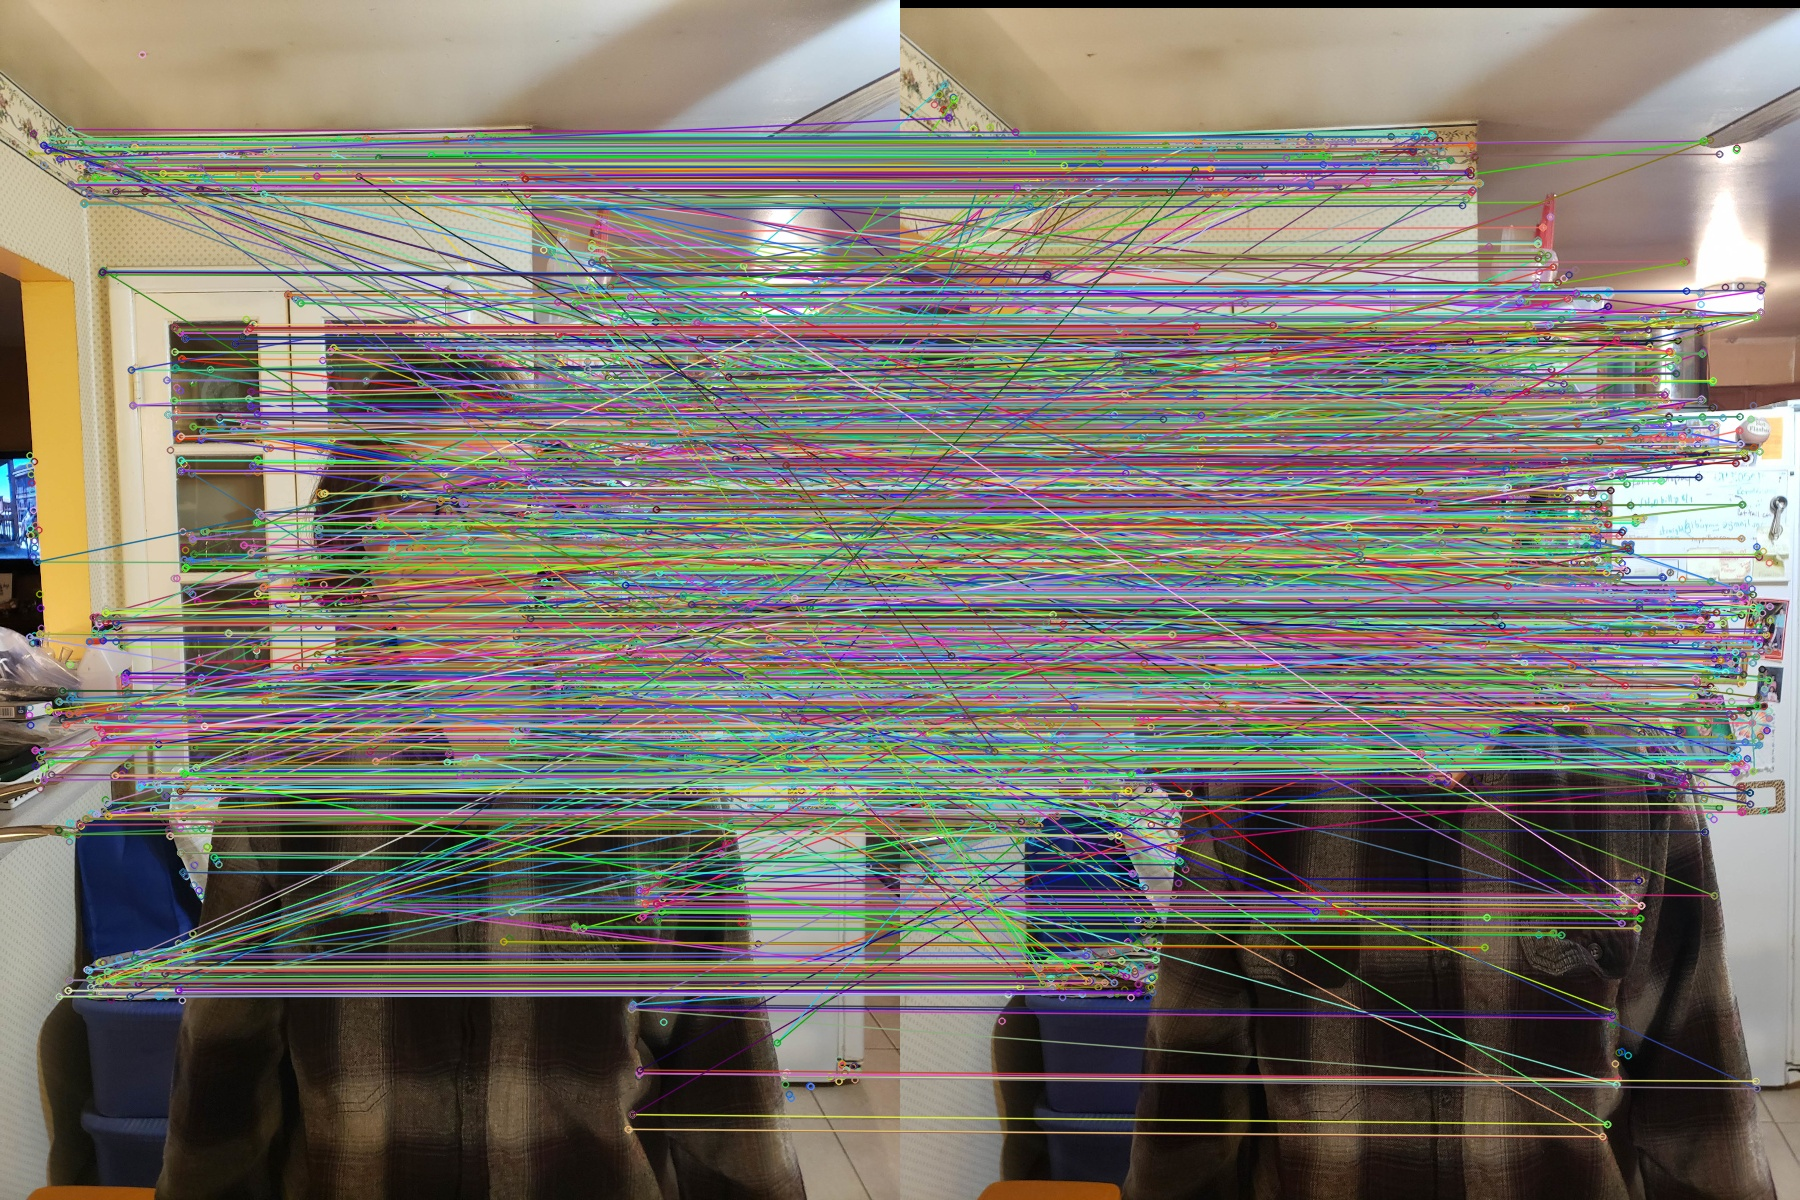
\includegraphics[width=3.0in]{bin/feature_matches.jpg} % Place holder, replace with \includegraphics, etc.
    \end{center}
    \caption{\small Feature matches between image 1 and 2, used to calculate the median transform for alignment.}
    \label{fig:features}
\end{figure}

\begin{figure*}[t!]
    \begin{subfigure}[t!]{\textwidth}
        \centering
        \begin{subfigure}[t]{0.33\textwidth}
            \centering
            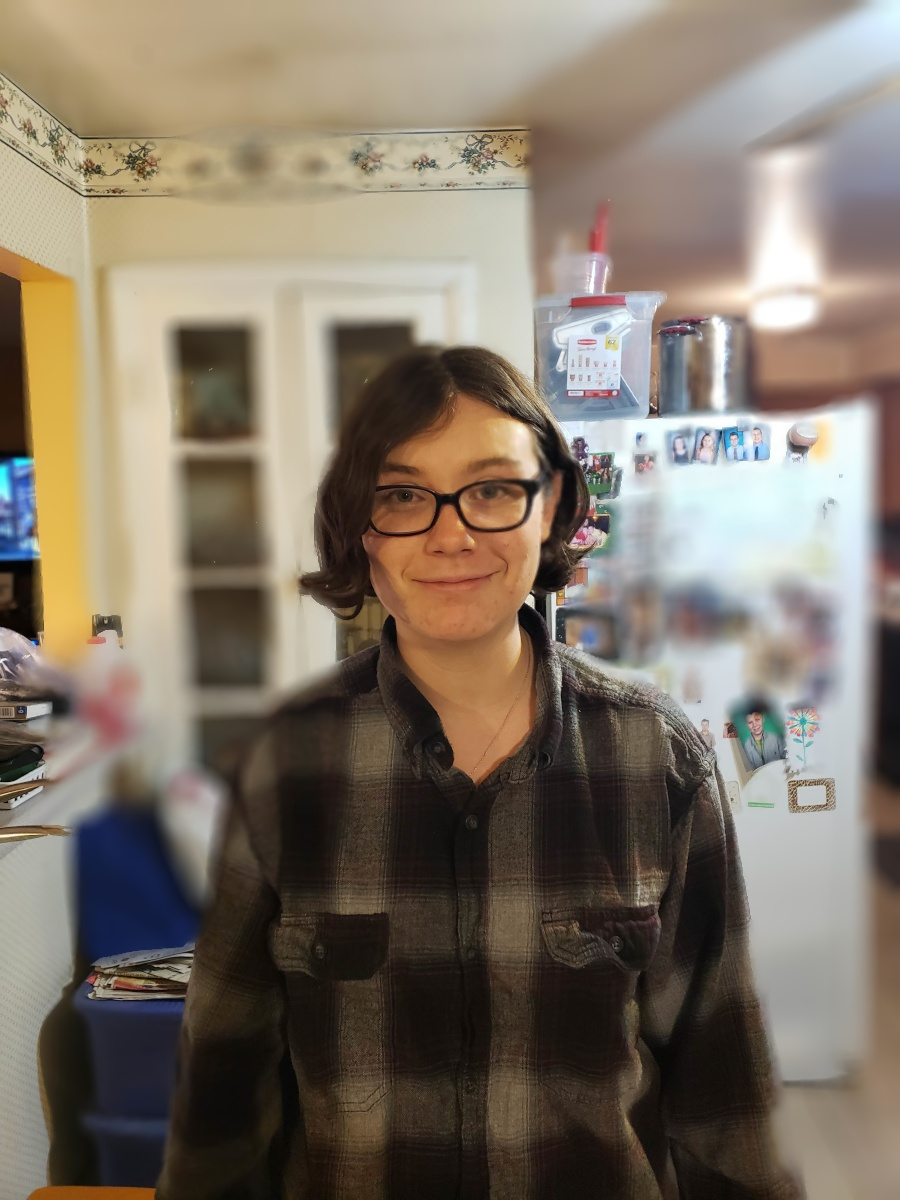
\includegraphics[width=1.2in]{bin/output_FBIL.jpg}
            \caption{Output using fast bilateral stereo}
        \end{subfigure}%
        ~
        \begin{subfigure}[t]{0.33\textwidth}
            \centering
            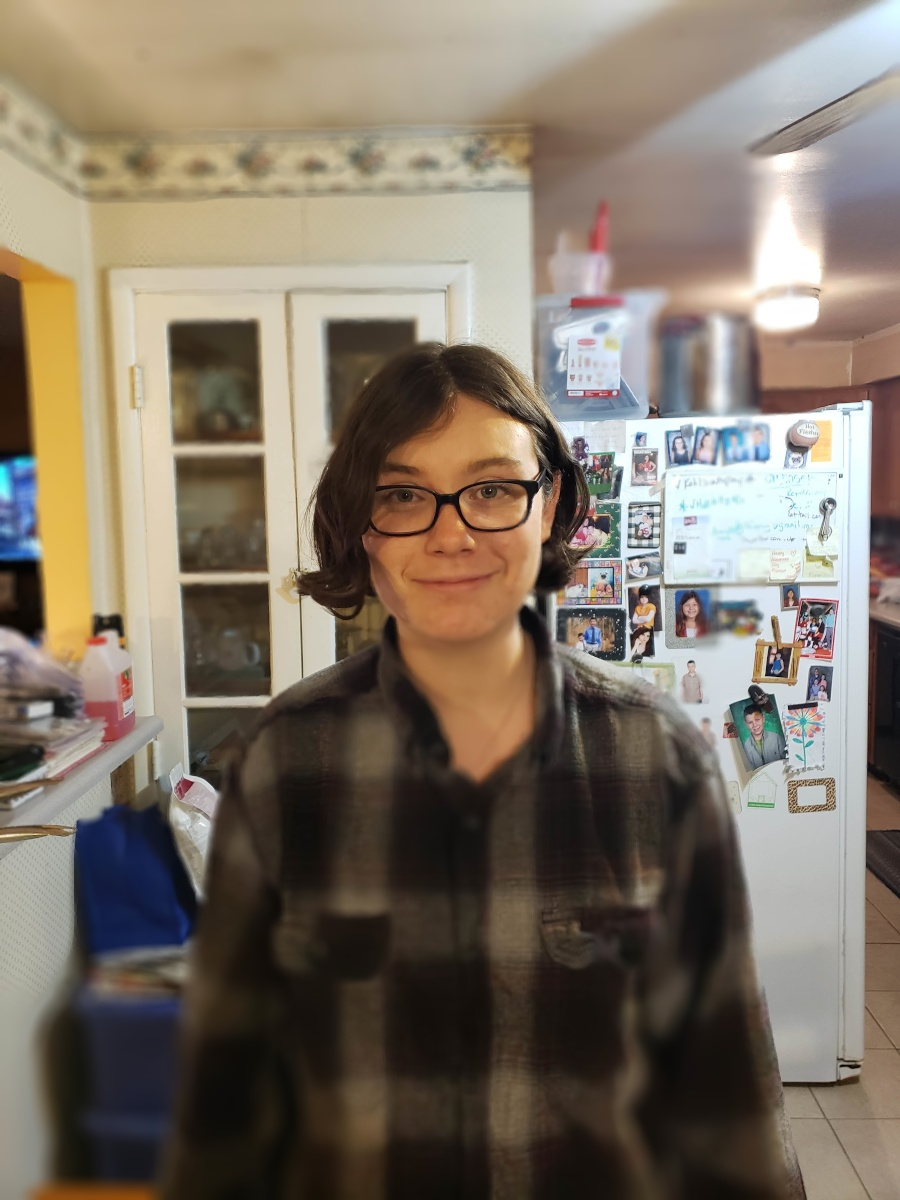
\includegraphics[width=1.2in]{bin/output_monodepth.jpg}
            \caption{Output using monodepth}
        \end{subfigure}%
        ~
        \begin{subfigure}[t]{0.33\textwidth}
            \centering
            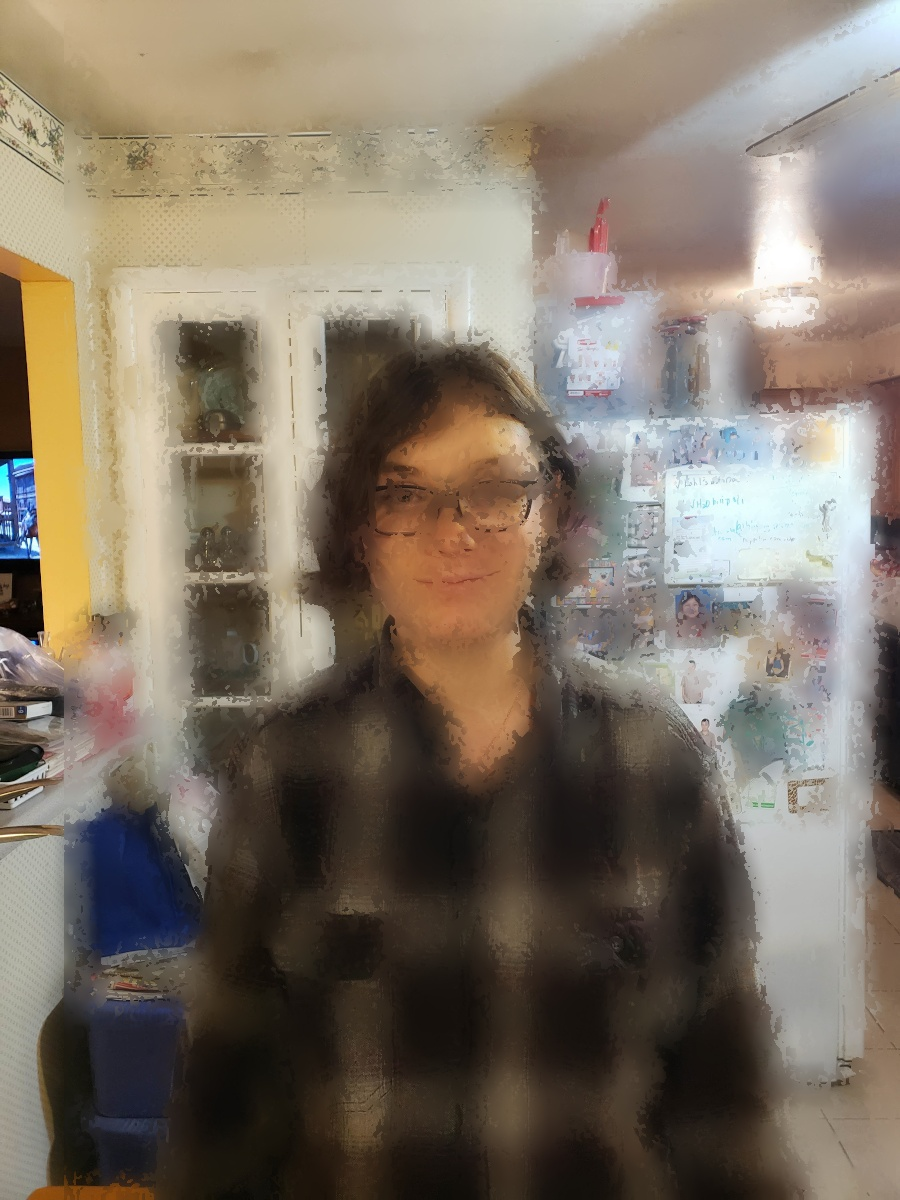
\includegraphics[width=1.2in]{bin/output_SGBM.jpg}
            \caption{Output using SGBM}
        \end{subfigure}
        \caption*{Output images using disc blurring with various methods}
    \end{subfigure}

    \begin{subfigure}[t!]{\textwidth}
        \centering
        \begin{subfigure}[t!]{0.33\textwidth}
            \centering
            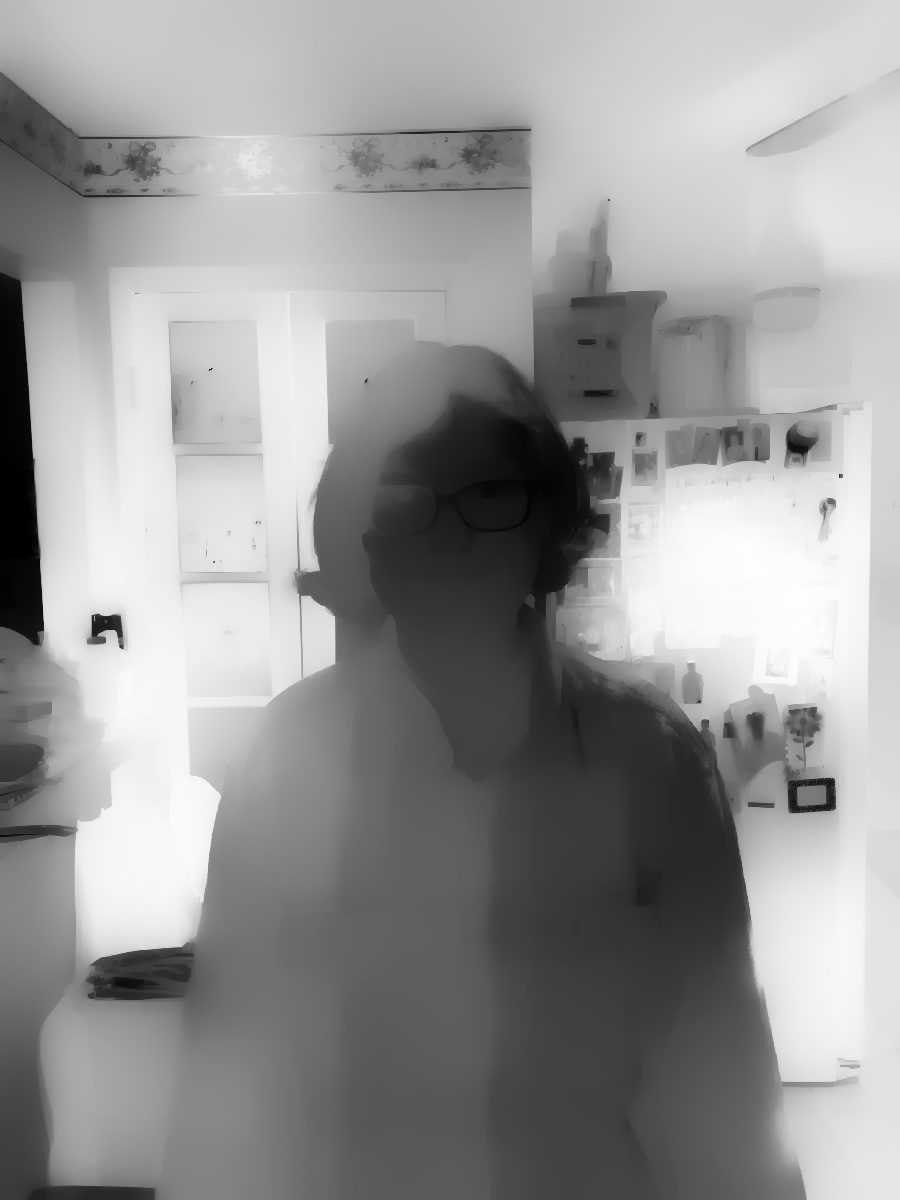
\includegraphics[width=1.2in]{bin/depth_map_FBIL.jpg}
            \caption{Depth map output from fast bilateral stereo}
        \end{subfigure}%
        ~
        \begin{subfigure}[t!]{0.33\textwidth}
            \centering
            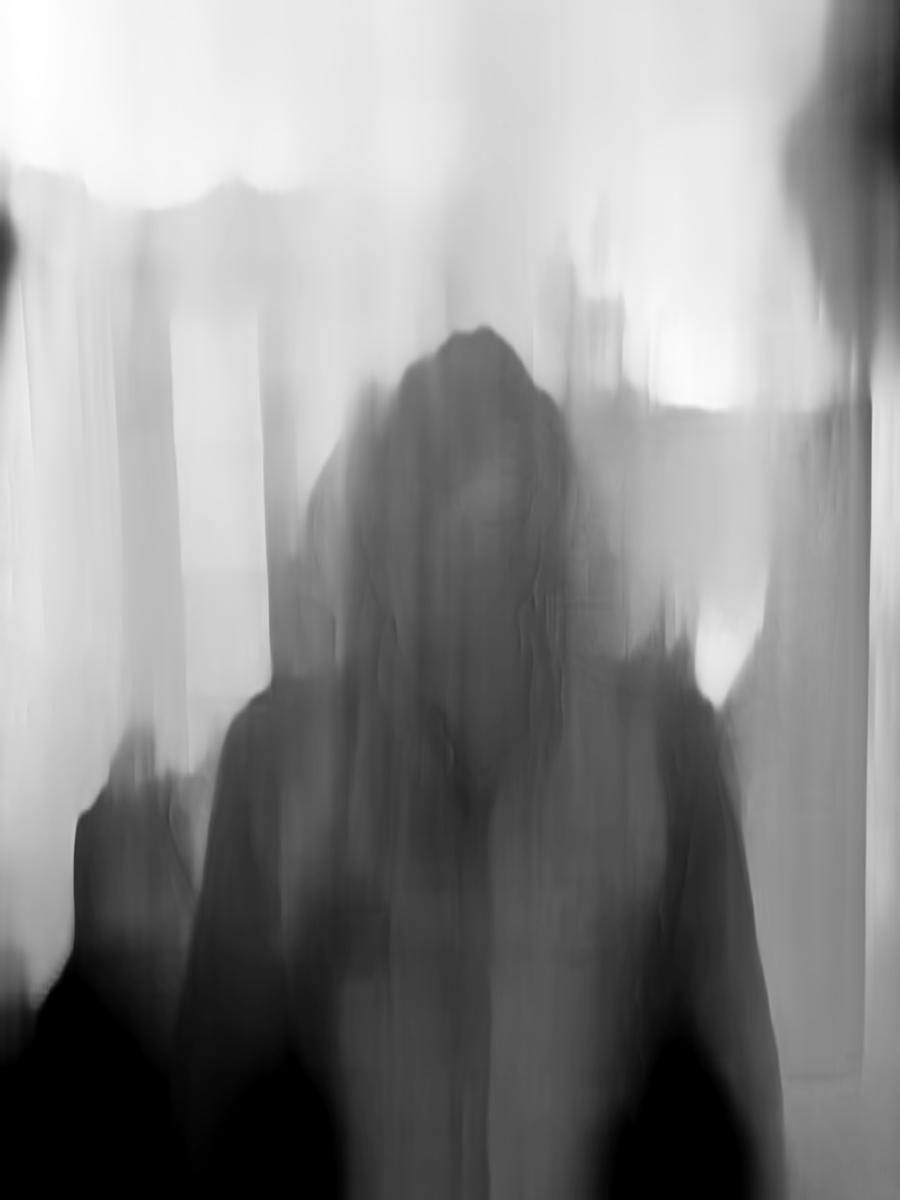
\includegraphics[width=1.2in]{bin/depth_map_monodepth.jpg}
            \caption{Depth map output from monodepth}
        \end{subfigure}%
        ~
        \begin{subfigure}[t!]{0.33\textwidth}
            \centering
            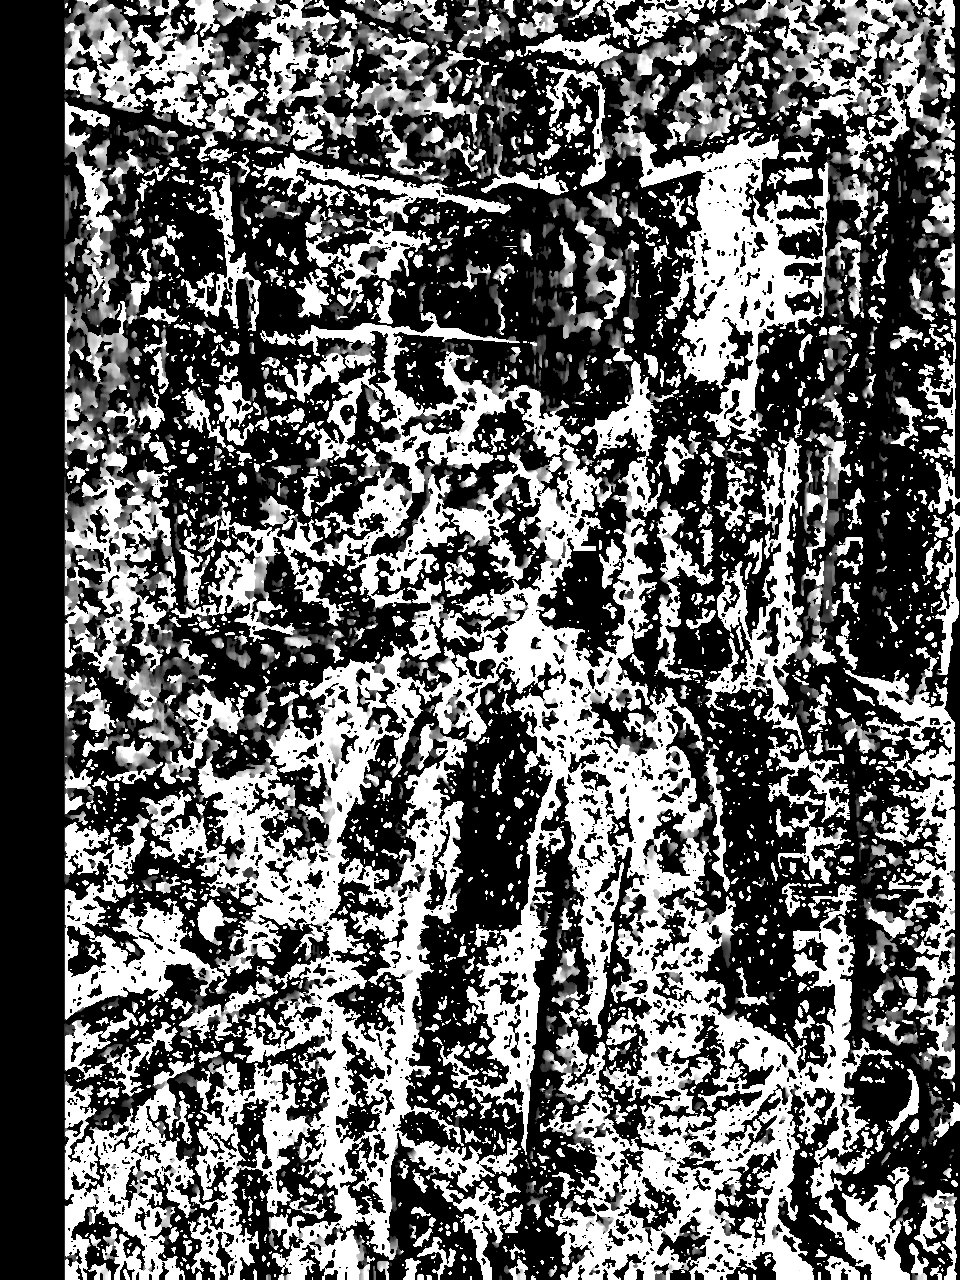
\includegraphics[width=1.2in]{bin/depth_map2_SGBM.jpg}
            \caption{Depth map output from SGBM}
        \end{subfigure}
        \caption*{Depth maps using various methods}
    \end{subfigure}

    \begin{subfigure}[t!]{\textwidth}
        \centering
        \begin{subfigure}[t!]{0.33\textwidth}
            \centering
            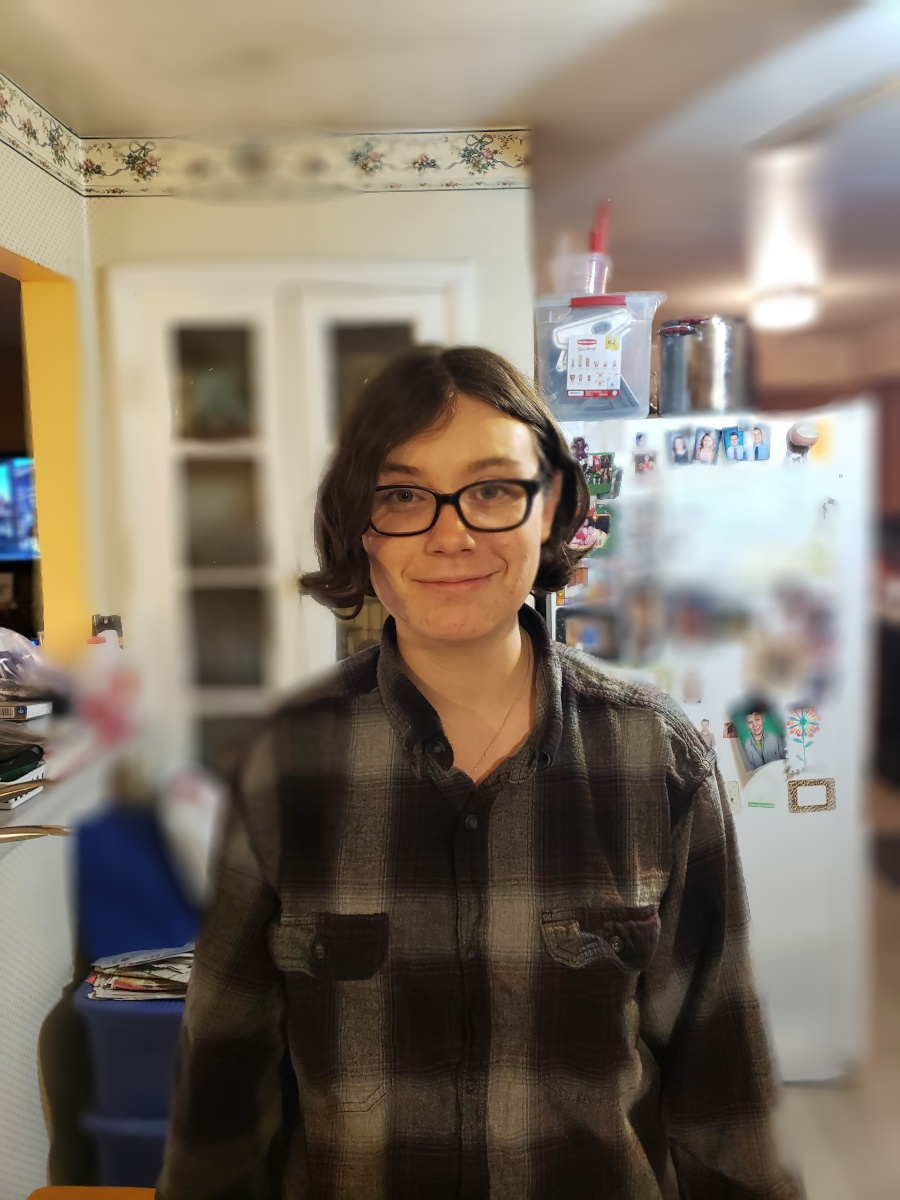
\includegraphics[width=1.2in]{bin/output_discblur.jpg}
            \caption{Output using disc blur}
        \end{subfigure}%
        ~
        \begin{subfigure}[t!]{0.33\textwidth}
            \centering
            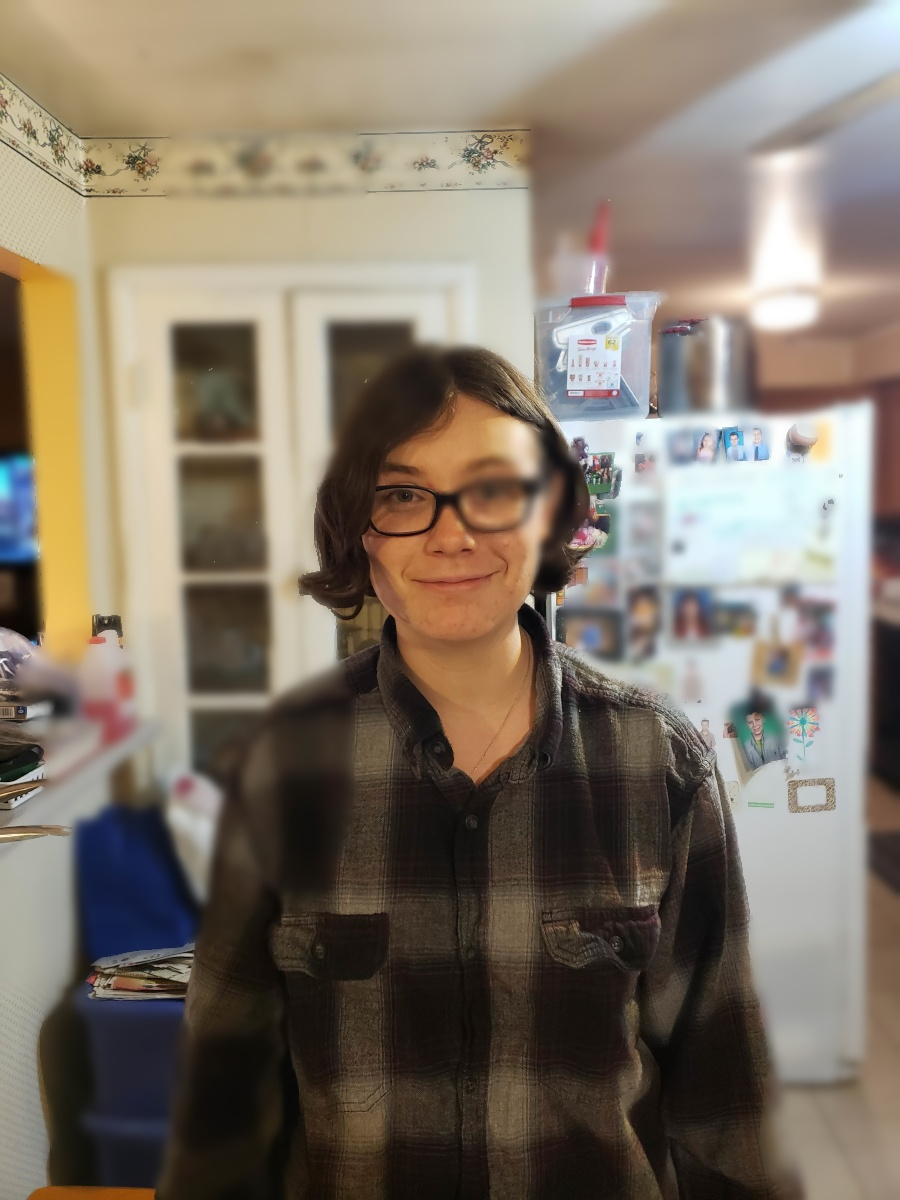
\includegraphics[width=1.2in]{bin/output_gaussianblur.jpg}
            \caption{Output using Gaussian blur}
        \end{subfigure}%
        ~
        \begin{subfigure}[t!]{0.33\textwidth}
            \centering
            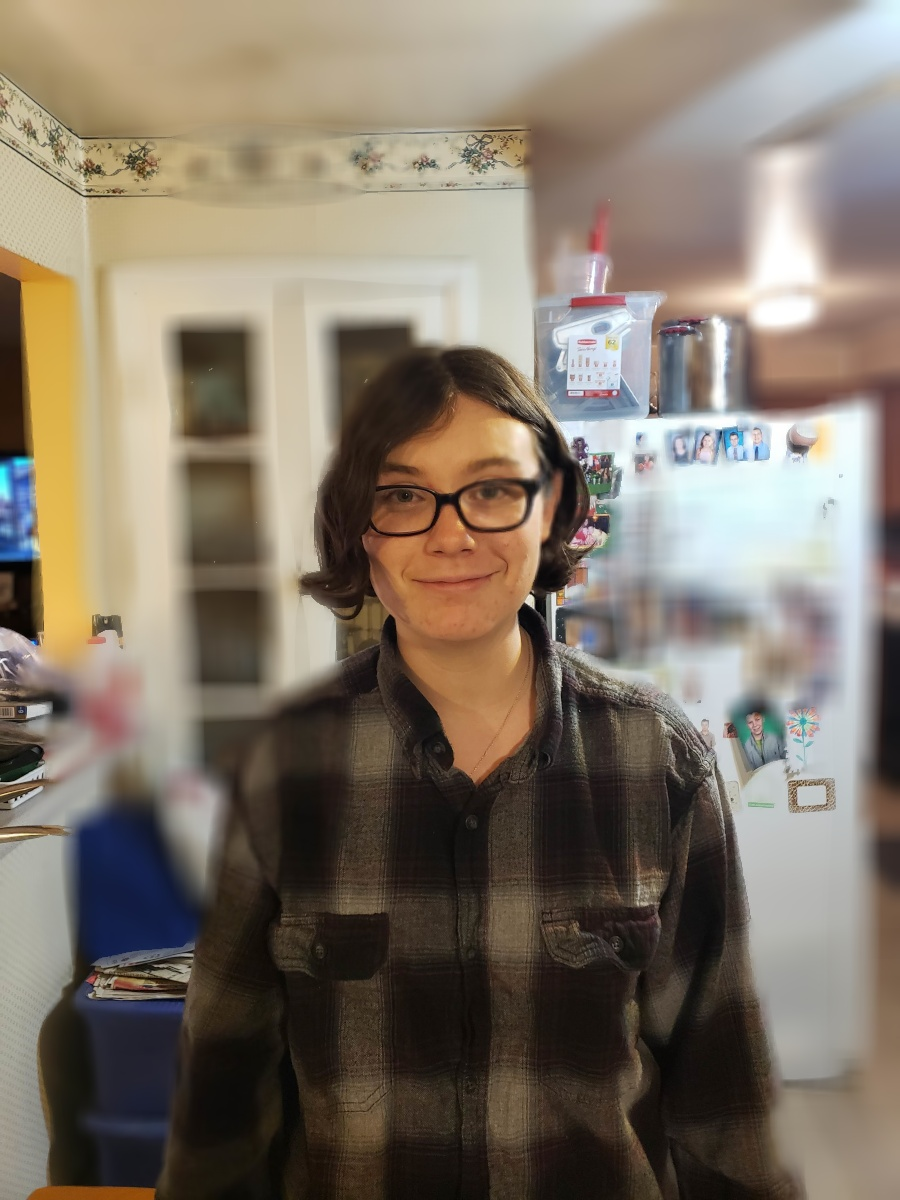
\includegraphics[width=1.2in]{bin/output_boxblur.jpg}
            \caption{Output using box filter blur}
        \end{subfigure}
        \caption*{Output images using fast bilateral stereo with various blurs}
    \end{subfigure}
    \caption{\small Example outputs using different blurring methods and stereo disparity matching algorithms, along with computed depth maps.
    Fast Bilateral Stereo Matching overall performed the best, but Monodepth2 performed surprisingly well given the automotive training data source.
    Disc blurring produced the most visually pleasing effect and was the closest to natural bokeh, but was computationally expensive and did not produce
    the characteristic "bokeh balls."}
    \label{fig:outputs}
\end{figure*}

\begin{figure*}[!t]
    \begin{subfigure}[t!]{\textwidth}
        \centering
        \begin{subfigure}[t]{0.33\textwidth}
            \centering
            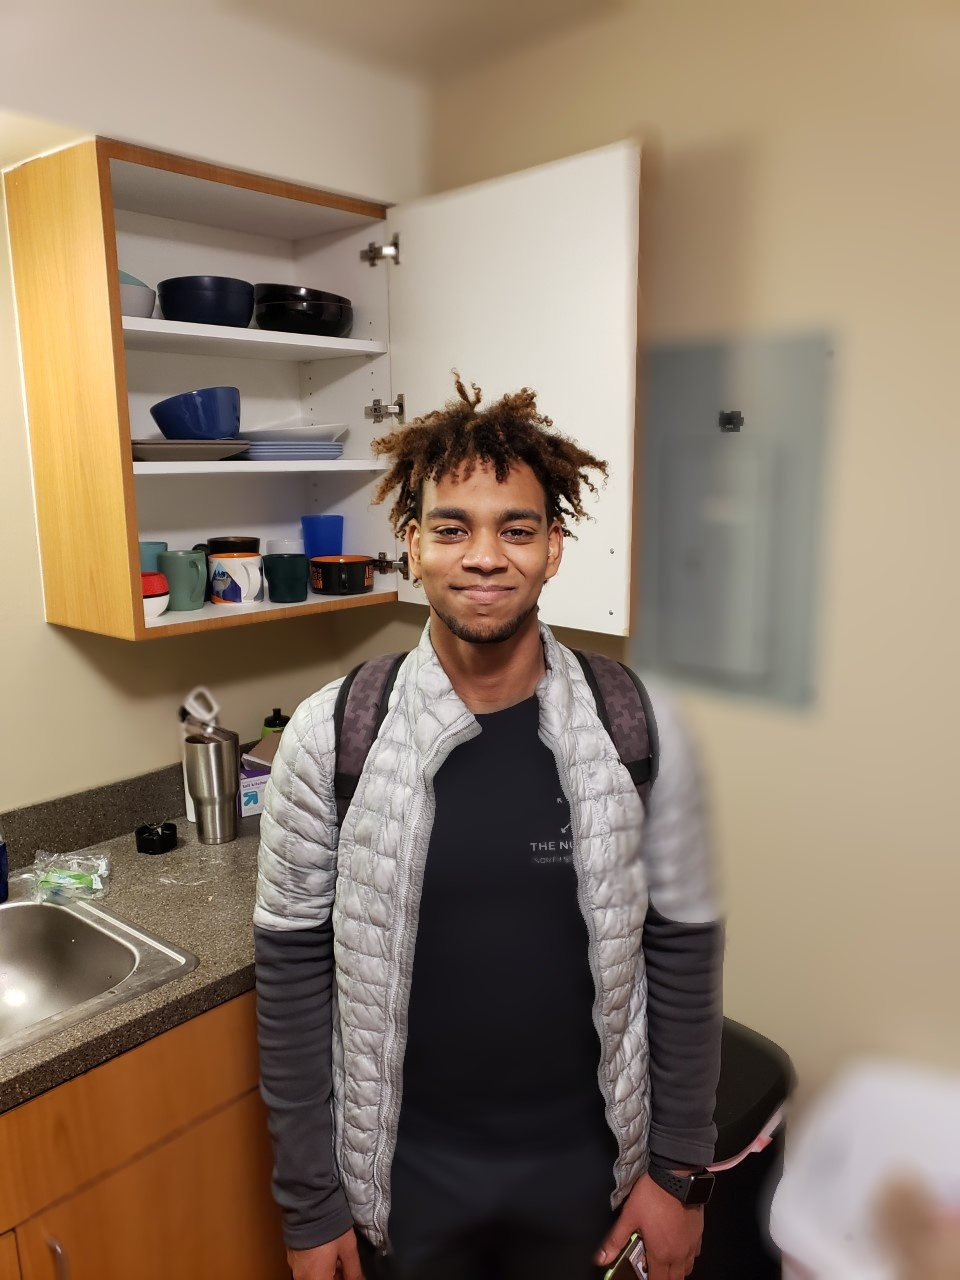
\includegraphics[width=1.2in]{bin/output2_FBIL.jpg}
            \caption{Output using fast bilateral stereo}
        \end{subfigure}%
        ~
        \begin{subfigure}[t]{0.33\textwidth}
            \centering
            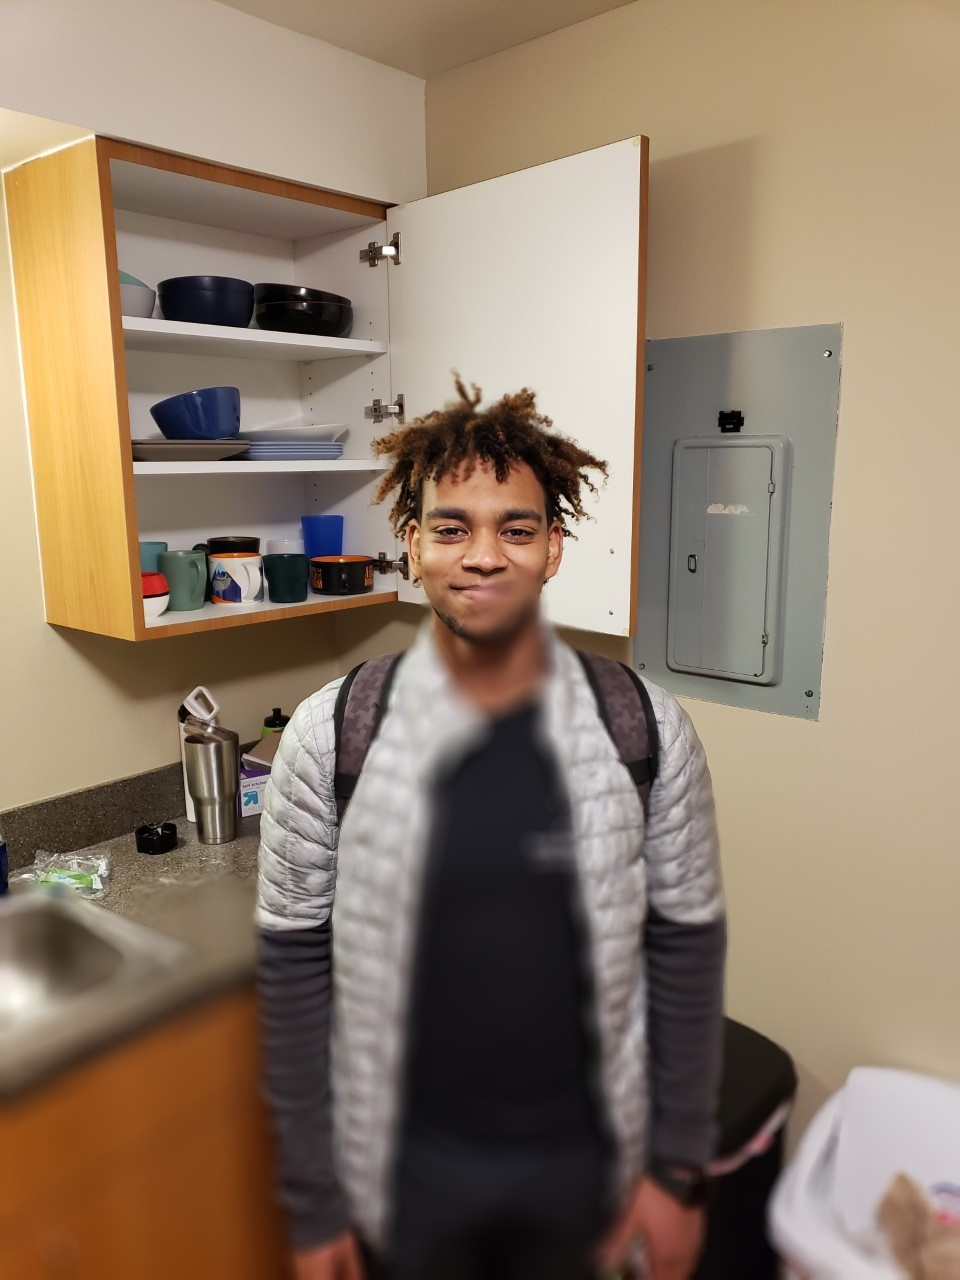
\includegraphics[width=1.2in]{bin/output2_monodepth.jpg}
            \caption{Output using monodepth}
        \end{subfigure}%
        ~
        \begin{subfigure}[t]{0.33\textwidth}
            \centering
            
\includegraphics[width=1.2in]{bin/output2_SGBM.jpg}
            \caption{Output using SGBM}
        \end{subfigure}
        \caption*{Output images using disc blurring with various methods on adversarial input.}
    \end{subfigure}
    \caption{\small Output from adversarial input. Input has sparse background, leading to extreme differences in disparity. In addition, the scene does not adhere to the enforced bilateral constraints, as the walls are not parallel to the sensor plane.}
    \label{fig:output2}
\end{figure*}

\section*{Acknowledgments}

Thanks to Toon Van den Zegel for his implementation of fast bilateral stereo. Additional thanks to Niantic, Inc. for monodepth2. Special thanks to Ella Gibson and Ahmed Hassan for helping provide input data.

{\small
\bibliographystyle{ieee}
\bibliography{refs} % Create file refs.bib, and run bibtex.
}

\end{document}
